\newpage
\begin{center}
  \textbf{\large 3. РАЗРАБОТКА ПРОГРАМНОГО ПРОДУКТА}
\end{center}
\refstepcounter{chapter}
\addcontentsline{toc}{chapter}{3. РАЗРАБОТКА ПРОГРАМНОГО ПРОДУКТА}

\section{Выбор инструментов разработки}
Первый этап процесса разработки заключался в выборе инструментов, которые будут использоваться в процессе разработки.

\textbf{IDE IntelliJ Idea} была выбрана в качестве рабочей среды для разработки сервисов.
Она предоставляет широкий набор функций и инструментов для разработки на языке Kotlin.

В качестве тестовой базы данных было решено использовать Docker-образ MongoDB. 
Docker-контейнер позволяет легко развернуть и настроить локальное окружение MongoDB, обеспечивая изолированную и портативную среду разработки. 

\textbf{Visual Studio Code} была выбрана в качестве рабочей среды для разработки мобильного приложения.
Она предоставляет широкий набор функций и инструментов для разработки на языке Dart.

\section{Процесс разработки сервисов}
\subsection{Общий модуль core}
Уже перед началом разработки было понятно, что сервисы будут иметь много схожей логики (модели данных, работа с БД, валидация данных, обработка ошибок, логирование и т.д.).
Поэтому для соблюдения принципа DRY 
\footnote{Don’t repeat yourself (DRY; с англ. — «не повторяйся») — это принцип разработки программного обеспечения, нацеленный на снижение повторения информации различного рода, особенно в системах со множеством слоёв абстрагирования.} 
было решено выделить общую часть в отдельный модуль, который будет подключаться к каждому сервису как зависимость. Данный модуль был назван \textbf{core}.
Структурная схема модулей и микросервисов представлена на рисунке \ref{fig:schemes:services}.

\begin{figure}
  \centering
  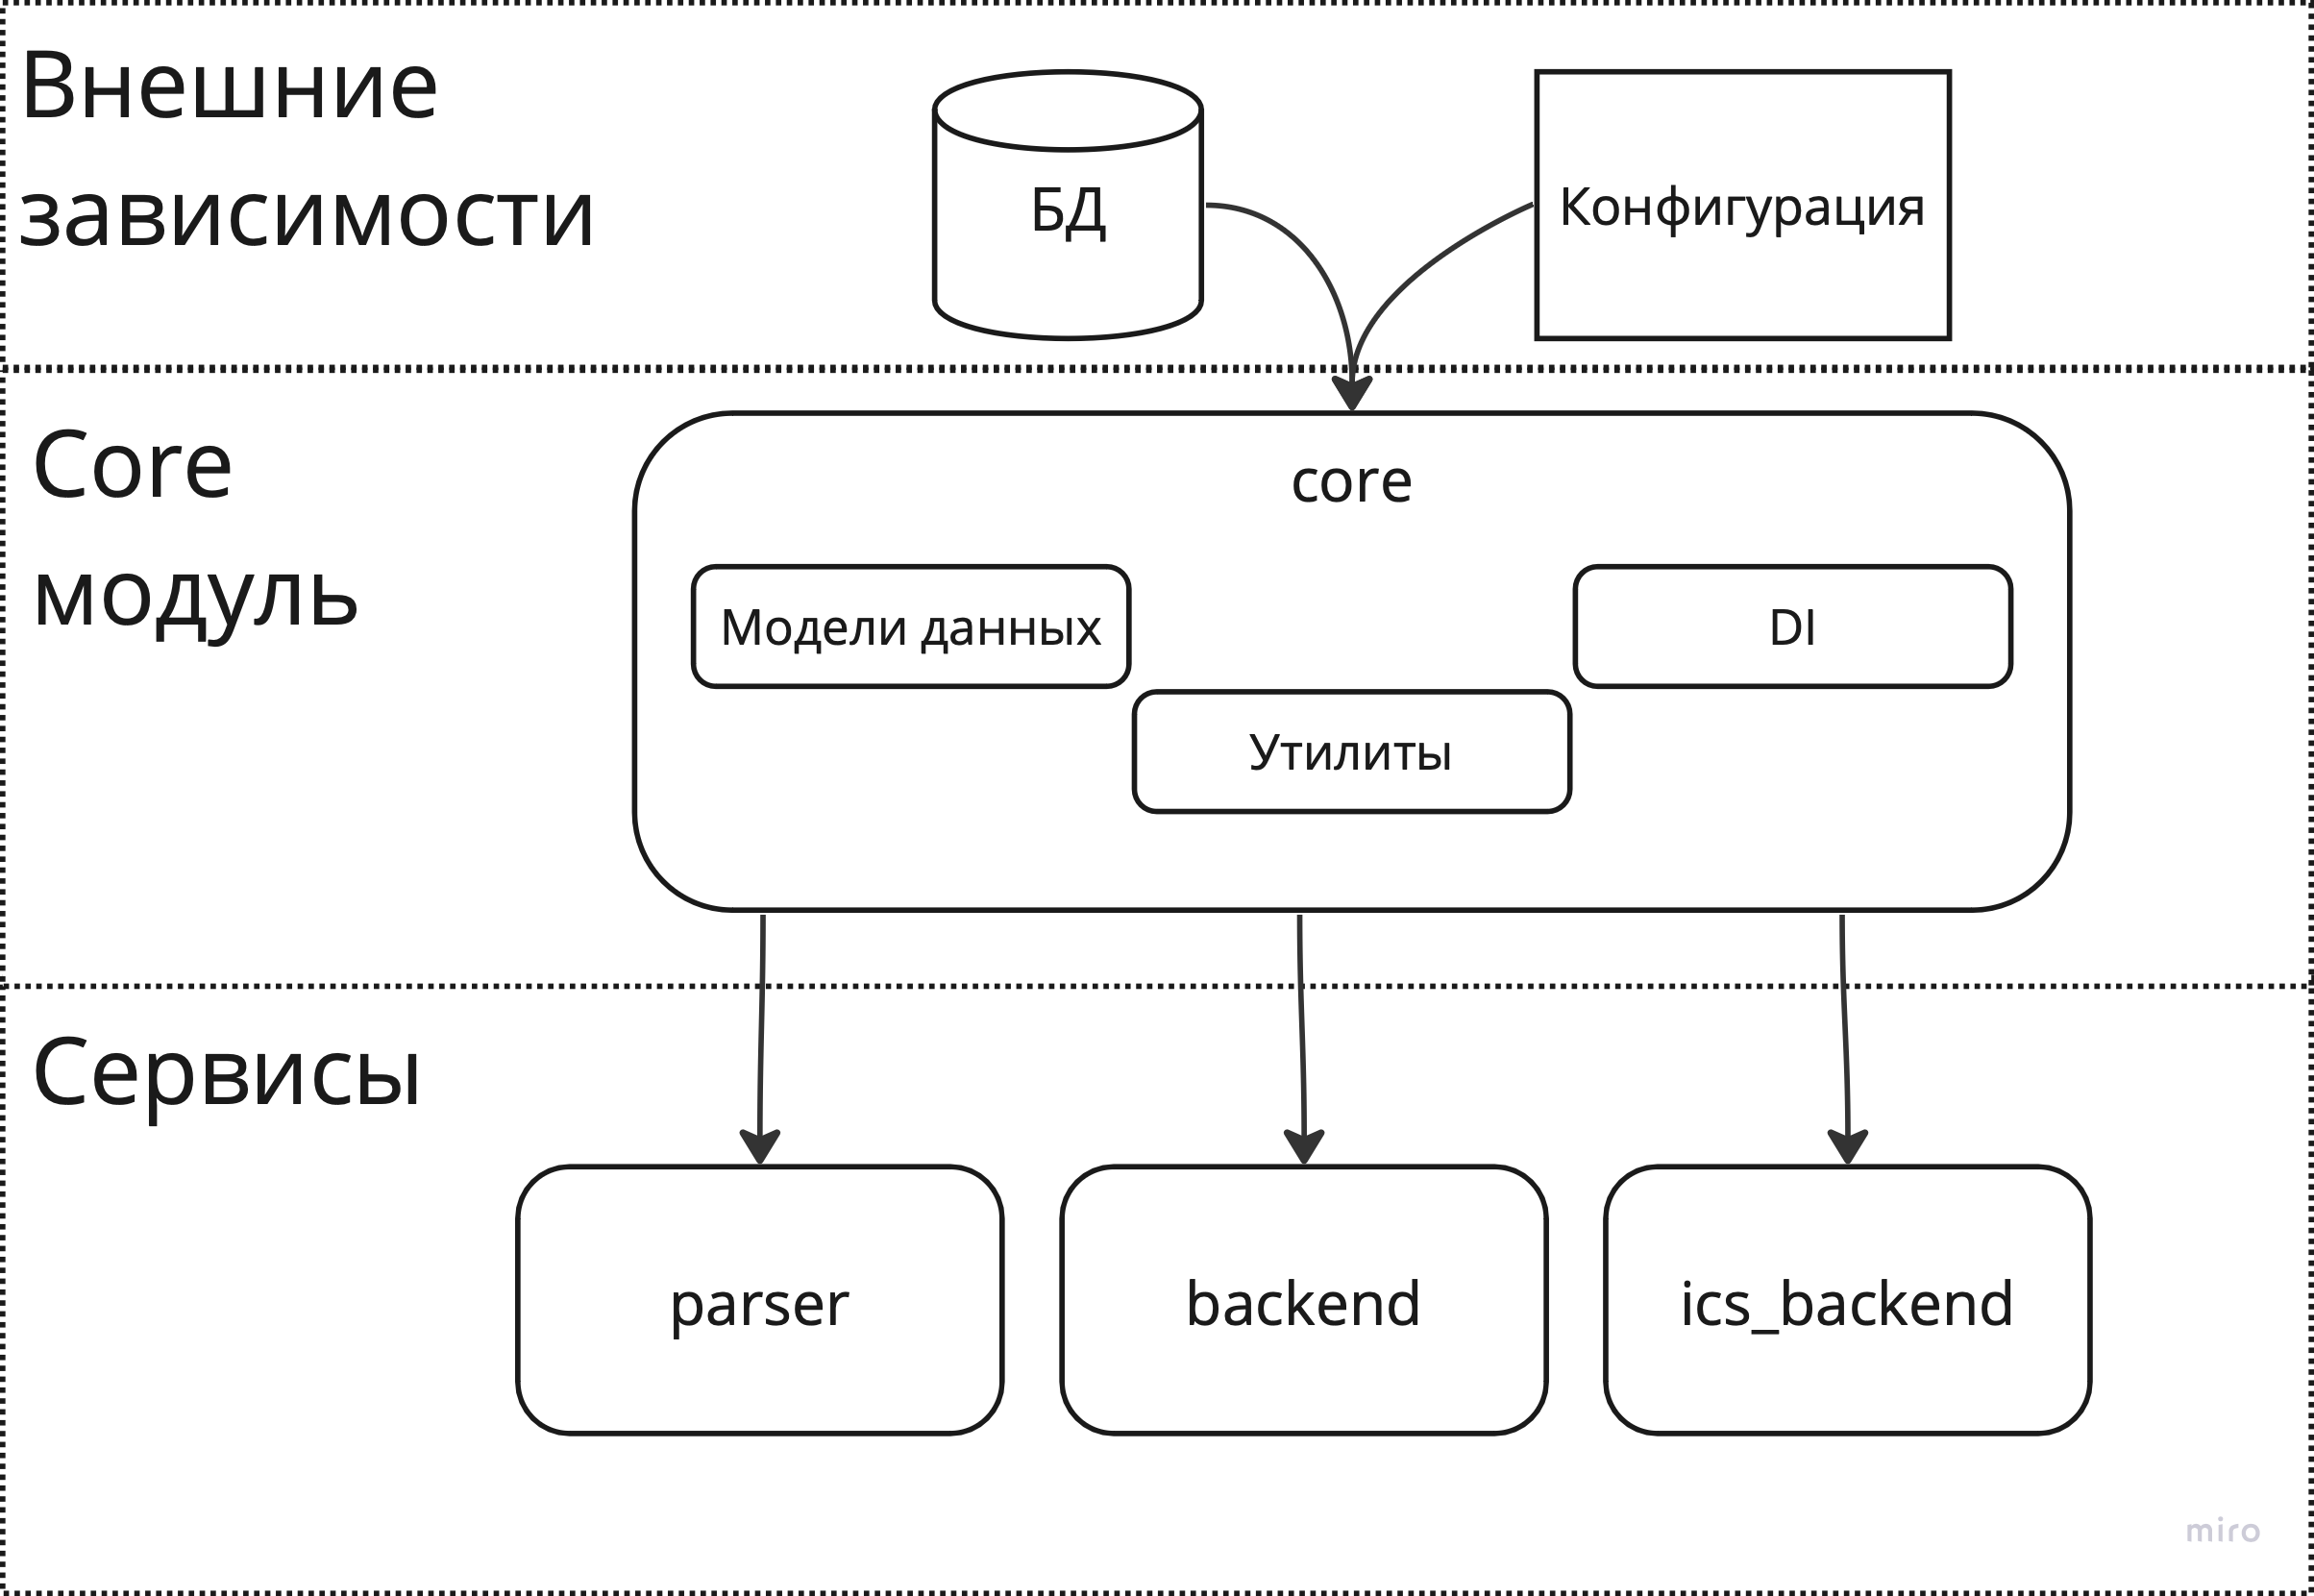
\includegraphics[width=0.8\linewidth]{images/schemes/services.png}
  \caption{Схема модулей серверной части. Линии показывают направление зависимостей.}
  \label{fig:schemes:services}
\end{figure}

Core модуль инкапсулирует в себе несколько функций: работа с данными, конфигурация, DI
\footnote{Dependency injection (DI) или внедрение зависимостей представляет механизм, который позволяет сделать компоненты программы слабосвязанными, 
а всю программу в целом более гибкой, более адаптируемой и расширяемой.
}, и предоставление общих внешних зависимостей.

Работа с данными включает себя описание моделей данных и репозиториев
\footnote{Репозиторий - это слой абстракции, инкапсулирующий в себе всё, что относится к способу хранения данных. 
Назначение: Разделение бизнес-логики от деталей реализации слоя доступа к данным.}
для работы с БД. Код моделей доступен по ссылке 4.1.\ref{code:models}.

\begin{enumerate}
  \item Модели данных - классы, которые описывают сущности, с которыми работает сервис (предмет, преподаватель, занятие, и т.д.).
  \item Общие внешние зависимости - библиотеки, которые используются в каждом сервисе (kmongo, koin, logback).
  \item Общие утилиты - классы, которые содержат вспомогательные функции (валидация данных, обработка ошибок, логирование и т.д.).
  \item Общший DI 

  контейнер - объект, который содержит в себе все зависимости, которые используются в разных сервисах.
  \item Общая конфигурация - класс, который содержит в себе конфигурацию приложения (порт, адрес БД, и т.д.).
\end{enumerate}



\section{Процесс разработки мобильного приложения}

\section{Развертывание АИС}

\section{Результаты разработки}